\chapter{Results and Analysis}
\label{ch:results}
\section{Performance Evaluation of Regression Models}
In this comprehensive analysis, we delve into the performance metrics of various regression models for predicting forest fire occurrences. Two distinct test sizes, 0.1 and 0.2, were considered to assess the models under different scenarios. Moreover, a series of preprocessing techniques were applied to the dataset before model training, aiming to enhance predictive accuracy.

\textbf{Test Size 0.1: Initial Insights}
At a test size of 0.1, the following models were evaluated:
\begin{itemize}
 \item \textbf{Linear Regression}: Despite its simplicity, the linear regression model achieved a moderate performance, with an MSE of 553.83 and an R2Score of 0.056.

 \item \textbf{XGBoost Regressor}: XGBoost, a popular gradient boosting algorithm, exhibited comparable results to linear regression, with an MSE of 559.21 and an R2Score of 0.047.

 \item \textbf{CatBoost Regressor}: The CatBoost algorithm, known for its robustness to categorical variables, yielded a slightly higher MSE of 599.77 and a negative R2Score of -0.022.

 \item \textbf{LightGBM Regressor}: LightGBM, another gradient boosting framework, showed the highest MSE of 919.30 and the lowest R2Score of -0.566 among the models evaluated.

 \item \textbf{Random Forest}: Employing a random forest model with default hyperparameters resulted in an MSE of 2.60 and a negative R2Score of -0.068.

 \item \textbf{Decision Tree}: The decision tree model, with specified hyperparameters, attained an MSE of 3.36 and a negative R2Score of -0.383.

 \item  \textbf{Tree}: Utilizing an extra tree regressor with preset hyperparameters yielded an MSE of 2.57 and a negative R2Score of -0.059.
 \end{itemize}
 
\textbf{Test Size 0.2: Detailed Examination}
Expanding the test size to 0.2 allowed for a more detailed examination of model performance, especially after preprocessing. The results for this configuration are as follows:
\begin{itemize}
\item \textbf{Linear Regression}: With extensive preprocessing, including one-hot encoding for day and month, binary encoding for the rain column, outlier removal, and log transformation of the area, linear regression demonstrated improved performance. The MSE decreased to 1.89, with a corresponding increase in the R2Score to 0.007.

\item \textbf{XGBoost Regressor}: Despite preprocessing, the XGBoost regressor's performance remained suboptimal, with an MSE of 2.04 and a negative R2Score of -0.073.

\item \textbf{CatBoost Regressor}: Similar to linear regression, CatBoost showed enhanced performance post-preprocessing, with an MSE of 1.89 and a marginally improved R2Score of 0.005.

\item \textbf{LightGBM Regressor}: While LightGBM demonstrated improved performance compared to XGBoost, its MSE of 1.98 and negative R2Score of -0.040 suggested room for further optimization.

\item \textbf{Random Forest}: The random forest model, after preprocessing, exhibited improved performance with an MSE of 1.98 and a negative R2Score of -0.040.

\item \textbf{Decision Tree}: With preprocessing, the decision tree model's MSE decreased to 2.92, accompanied by a negative R2Score of -0.537.

\item \textbf{Extra Tree}: Preprocessing enhanced the extra tree regressor's performance, with an MSE of 1.89 and a positive R2Score of 0.007.
\end{itemize} 

\clearpage
\section{Feature Selection and Preprocessing}
Before model training, several preprocessing steps were undertaken to optimize feature selection and enhance model interpretability. In figure 4 Positive values indicate positive correlation, while negative values indicate negative correlation. Among the features, temperature (temp) shows the strongest positive correlation with the target variable, while relative humidity (RH) demonstrates the weakest correlation.

\begin{figure}[ht]
    \centering
    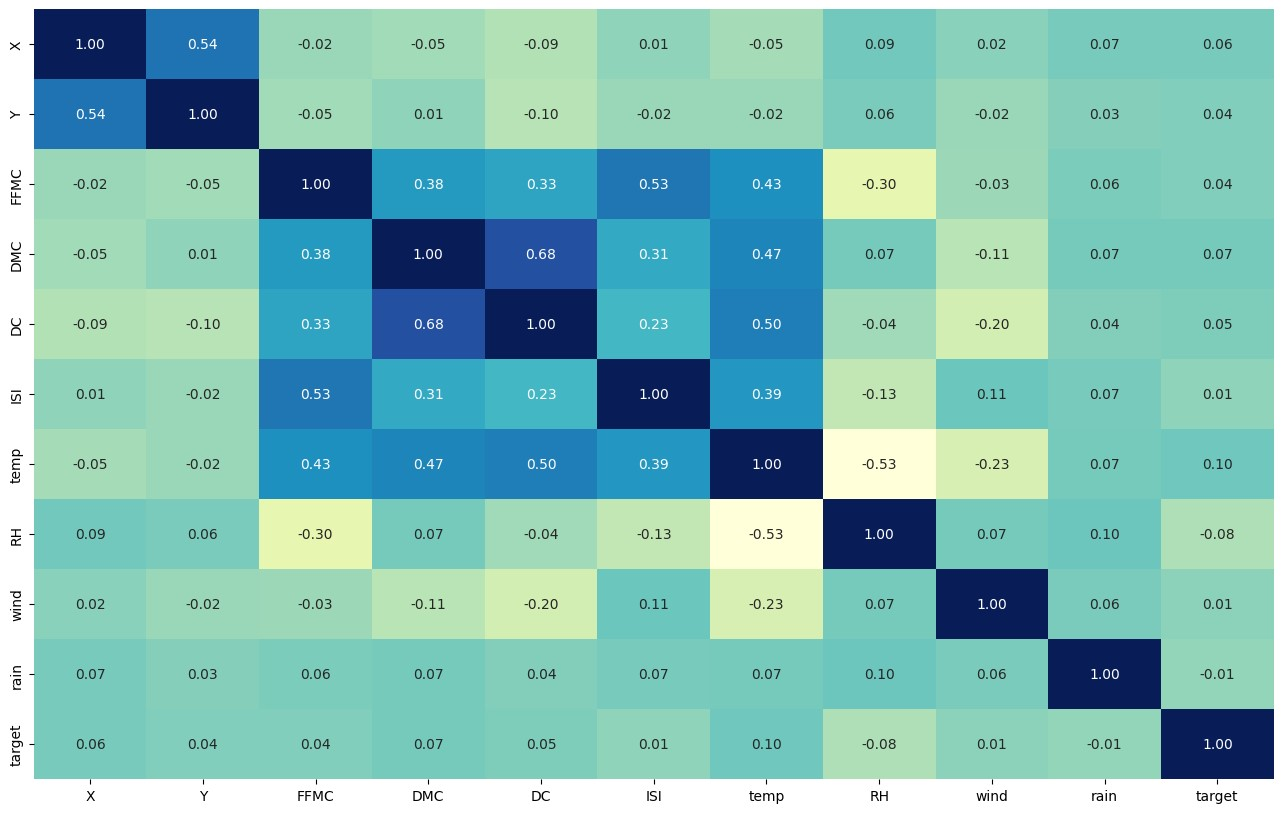
\includegraphics[scale=0.5]{figures/Correlation Matrix.jpg}
    \caption{Figure 2: Correlation Matrix: This matrix displays the correlation coefficients between variables, including spatial coordinates, meteorological factors, and the target variable (forest fire volume). }
    \label{fig:example-01}
\end{figure}

\clearpage
\textbf{One-Hot Encoding}: Categorical variables such as day and month were transformed into numerical form through one-hot encoding, enabling their integration into the regression models

\begin{figure}[ht]
    \centering
    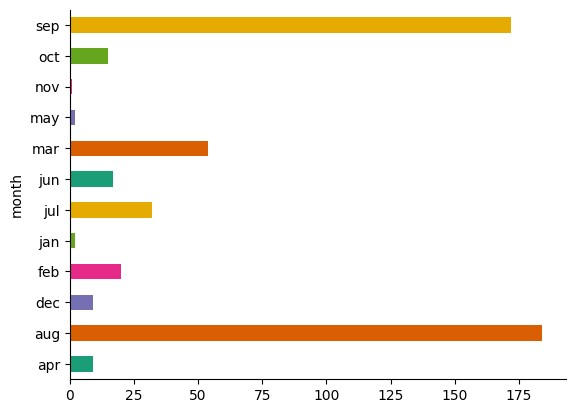
\includegraphics[scale=0.8]{figures/Monthly Distribution of Forest fire.jpg}
    \caption{Figure 3: Monthly distribution of forest fire volume in the study area, Alto Minho.The image illustrates the volume of forest fires recorded in each month, highlighting August and September as peak months
}
    \label{fig:example-01}
\end{figure}

\textbf{Binary Encoding}: Binary encoding was applied to the rain column, simplifying its representation and facilitating its inclusion in the regression models.

\textbf{Outlier Removal}: Data points that deviated significantly from the dataset's distribution were identified as shown in figure 4.3 and removed to prevent them from skewing model predictions.

\begin{figure}[ht]
    \centering
    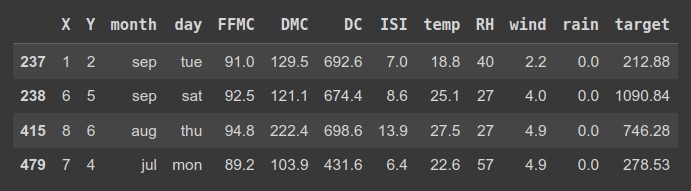
\includegraphics[scale=0.9]{figures/Outlier Records.jpg}
    \caption{Table 3: Outlier Records :Representative outliers displaying spatial coordinates, month, day, meteorological indices, and target variable values from the dataset}
    \label{fig:example-02}
\end{figure}

\textbf{Log Transformation}: The target variable, area, underwent log transformation to achieve a more symmetric distribution and stabilize variance, a common practice in linear regression problems.






